\section{Experiments}
\label{sec:experi}

\subsection{Experimental Setup}

\noindent\textbf{Evaluated Models.}
We evaluate 13 frontier proprietary and open-source LLMs. The proprietary models include OpenAI’s GPT-5 and GPT-5-mini; Google’s Gemini-2.5-Pro and Gemini-2.5-Flash; and Anthropic’s Claude-4.5-Sonnet. The open-source models include DeepSeek’s DeepSeek-V3.1; Alibaba’s Qwen3 (8B/32B) and Qwen-2.5 (7B/32B/72B); and Meta’s Llama-3.3-70B and Llama-3.1-8B.

\noindent\textbf{Prompting Methods.}
We evaluate two baseline prompting methods: Standard Prompting and Step-by-Step Prompting. In Standard Prompting, the model receives the query and the full trajectory and is asked to perform hallucination judgment and attribution. In Step-by-Step Prompting, the model receives the query and the trajectory incrementally and determines at each step whether a hallucination occurs, terminating immediately upon detection. More details can be found in Appendix~\ref{appendix_evaluation_method}.

\noindent\textbf{Evaluated Metrics.}
For hallucination judgment, we evaluate binary classification performance using standard metrics, including macro-F1, macro-recall, and accuracy.
For hallucination attribution, we report step localization accuracy, defined as the proportion of hallucinated instances for which the model correctly identifies the responsible step.
In addition, we use G-EVAL~\cite{liu2023g} with GPT-5 as the evaluator to score explanation quality. More details can be found in Appendix~\ref{appendix_evaluation_metric}.

\subsection{Main Results}

\begin{figure*}[!t]
  \centering
    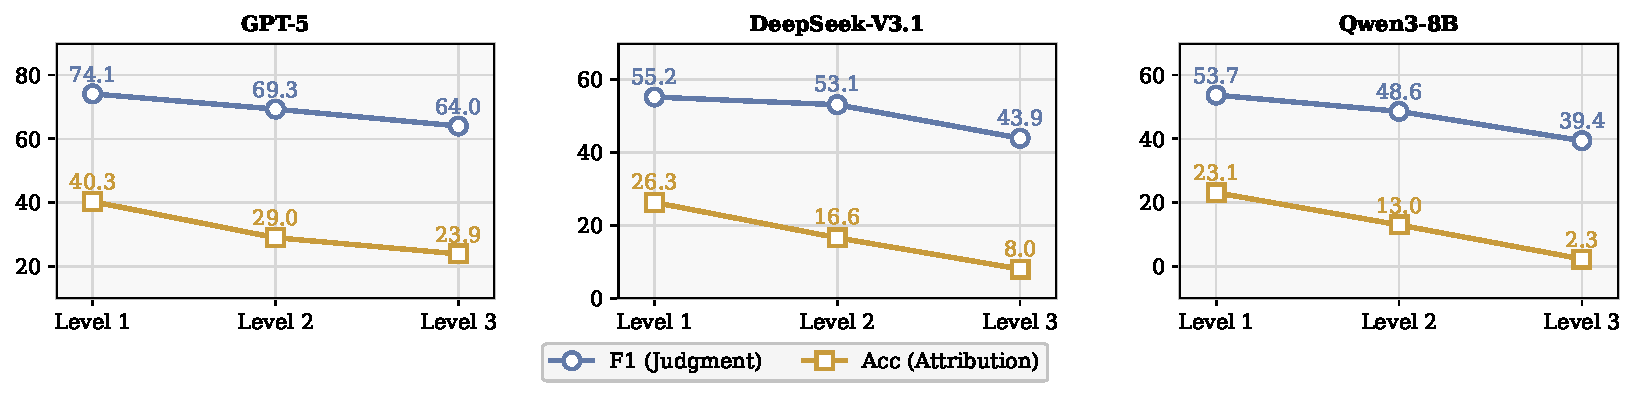
\includegraphics[width=1.0\linewidth]{Fig/agent_length.pdf}
    \vspace{-1.8em}
    \caption{Comparison of hallucination judgment and attribution performance across LLMs under varying trajectory steps $N_{\text{step}}$. Level 1 spans trajectories with $N_{\text{step}} \le 5$, Level 2 spans $6 \le N_{\text{step}} \le 10$, and Level 3 spans $N_{\text{step}} \ge 11$.
    }
    \label{fig:agent_length}
\end{figure*}

\paragraph{Comparison of Different LLMs.} Table~\ref{model_comparision} reports the main results of different LLMs on AgentHallu. Our key findings are summarized as follows:

\textit{(1) Challenges of Attribution}: A substantial performance gap remains between hallucination judgment and attribution tasks. While advances in proprietary models have boosted judgment performance to a peak F1 of 70.2\% for GPT-5, the more demanding attribution task reaches only 41.1\% localization accuracy and a 2.4 G-EVAL score for Gemini-2.5-Pro. These results indicate considerable room for attribution improvement and highlight the rigorous standards of this benchmark.

\textit{(2) Disparity between Proprietary and Open-source Models}: Open-source models achieve an average localization accuracy of 10.9\%, a level comparable to a random baseline and substantially below 35.9\% of proprietary models. Even the strongest open-source model, DeepSeek-V3.1, attains only 19.2\% localization accuracy. This performance gap may be attributed to the limited reasoning capabilities of open-source models.

\textit{(3) Category-level Analysis}:
Attribution accuracy varies substantially across hallucination categories. Reasoning hallucinations are comparatively easier to localize, with Gemini-2.5-Pro reaching 64.4\% accuracy, whereas tool-induced hallucinations remain consistently the most difficult across all model families. This may be attributed to the challenge of verifying environmental state within action–observation loops, rather than purely linguistic factual errors. Further analysis on subcategories is provided in Appendix~\ref{appendix_subcategory_analysis}.

\begin{table}[!ht]
  \centering
%   \scriptsize
  \caption{Comparison of prompting methods in terms of hallucination judgment (Judg.) F1, attribution (Attr.) step localization accuracy, and inference token cost.}
      \vspace{-0.5em}
  \label{method_comparision}
    \resizebox{1.0\linewidth}{!}{
    \tablestyle{5.0pt}{1.1}
   \begin{tabular}{c|c|c|c|c}
\toprule
\rowcolor{COLOR_MEAN} 
\cellcolor{COLOR_MEAN}                                                                                 & \cellcolor{COLOR_MEAN}                                                                                      & \textbf{Judg.} & \textbf{Attr.} & \textbf{Efficiency} \\ \cline{3-5} 
\rowcolor{COLOR_MEAN} 
\multirow{-2}{*}{\cellcolor{COLOR_MEAN}\textbf{\begin{tabular}[c]{@{}c@{}}Model \\ Name\end{tabular}}} & \multirow{-2}{*}{\cellcolor{COLOR_MEAN}\textbf{\begin{tabular}[c]{@{}c@{}}Prompting\\ Method\end{tabular}}} & \textbf{F1}$\uparrow$       & \textbf{Acc}$\uparrow$         & \textbf{Token Cost} \\ \midrule \midrule
                                                                                                         & Standard                                                                                                      & \textbf{70.2}     & 32.7                 & 7,426               \\
\multirow{-2}{*}{GPT-5}                                                                                  & Step-by-Step                                                                                                  & 68.5              & \textbf{42.7}        & \textbf{25,454}     \\ \midrule
                                                                                                         & Standard                                                                                                      & \textbf{52.1}     & 19.0                 & 6,494               \\
\multirow{-2}{*}{\begin{tabular}[c]{@{}c@{}}DeepSeek\\ -V3.1\end{tabular}}                               & Step-by-Step                                                                                                  & 51.1              & \textbf{35.9}        & \textbf{11,457}     \\ \midrule
                                                                                                         & Standard                                                                                                      & 51.8              & 21.2                 & 5,017               \\
\multirow{-2}{*}{\begin{tabular}[c]{@{}c@{}}Qwen3\\ -32B\end{tabular}}                                   & Step-by-Step                                                                                                  & \textbf{52.2}     & \textbf{31.2}        & \textbf{15,630}     \\ \bottomrule
\end{tabular}
}
\end{table}



\paragraph{Comparison of Different Prompting Methods.}
We compare two prompting methods for hallucination judgment and attribution in Table~\ref{method_comparision}.
For hallucination judgment, the standard prompt remains consistently competitive and slightly outperforms the step-by-step variant, suggesting that binary decisions benefit from aggregating evidence over the full trajectory. In contrast, the step-by-step method substantially improves attribution, raising accuracy from 24.3\% to 36.6\% on average by incrementally processing context to enable more focused step localization. However, this method comes at a clear efficiency trade-off, increasing the average input token cost from 6,312 to 17,514 due to the additional decisions with multi-turn prompting.

\paragraph{Performance across Varying Trajectory Steps.}
To further examine the effect of trajectory steps on hallucination diagnosis, we partition the trajectory logs from AgentHallu into three levels based on the number of steps $N_{\text{step}}$. Level 1 includes trajectories with $N_{\text{step}} \le 5$, Level 2 covers $6 \le N_{\text{step}} \le 10$, and Level 3 contains $N_{\text{step}} \ge 11$, resulting in 278, 274, and 141 samples, respectively. Both judgment and attribution performances for three LLMs across these levels are presented in Figure~\ref{fig:agent_length}. The results show a consistent degradation in both tasks as trajectory length increases. Notably, attribution accuracy drops significantly on average, from 29.9\% at Level 1 to 11.4\% at Level 3, suggesting that the accumulation of distracting context can effectively obscure the hallucination-responsible step.



\begin{figure*}[!ht]
  \centering
    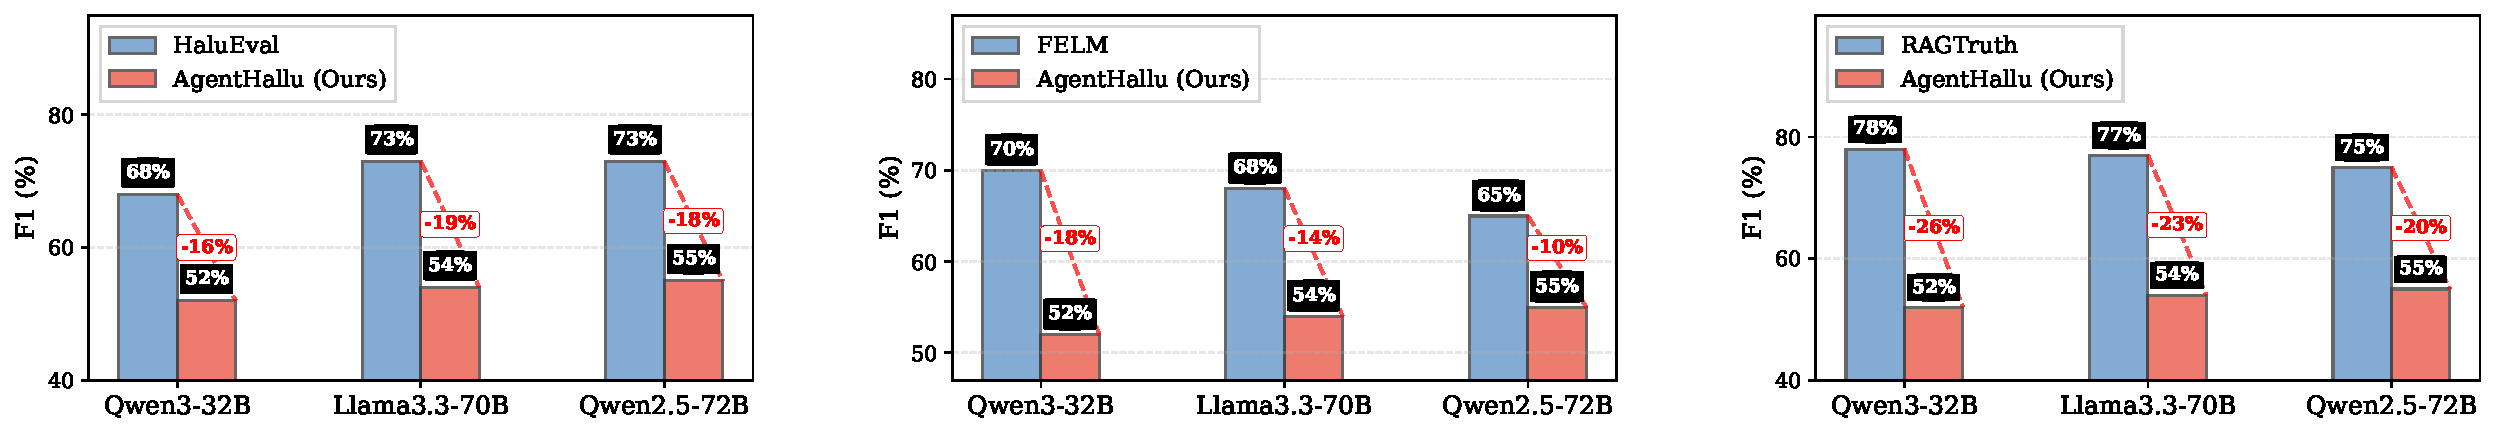
\includegraphics[width=1.0\linewidth]{Fig/dataset_comparison.pdf}
    \vspace{-1.8em}
    \caption{ Comparison of hallucination judgment F1 (\%) on AgentHallu against existing hallucination detection datasets across multiple LLMs.
    }
    \label{fig:hallu_dataset}
\end{figure*}

\begin{table}[ht!]
    \centering
    \caption{Spearman and Kendall-Tau correlations between different metrics and human annotations.}
    \vspace{-0.5em}
    \label{evaluation_consistency}
    \resizebox{\linewidth}{!}{
    \tablestyle{3.0pt}{1.1}
    \begin{tabular}{l||cc}
\toprule
\rowcolor{COLOR_MEAN} 
\textbf{Evaluation Metric} & \textbf{Spearman} & \textbf{Kendall-Tau} \\ \midrule
Rouge-L           &0.44           &0.34              \\
BERTScore         &0.32           &0.24              \\
G-EVAL-Qwen3-32B  &0.78           &0.62              \\
G-EVAL-GPT5       &\textbf{0.86}           &\textbf{0.76}              \\ \bottomrule
\end{tabular}
    }
\end{table}

\paragraph{Human Evaluation on Explanations.}
To examine alignment between causal explanation evaluation and human preference, we conduct a user study on 100 curated trajectory–explanation pairs from AgentHallu. The pairs are uniformly sampled across five hallucination categories and span outputs from five models, including GPT-5, Gemini-2.5-Pro, DeepSeek-V3.1, Qwen3-32B, and Llama3.3-70B. Three annotators with AI expertise independently rate each pair on a five-point scale. In Table~\ref{evaluation_consistency}, LLM-based evaluator, G-EVAL, align more closely with human judgments than Rouge-L~\cite{lin2004rouge} and BERTScore~\cite{zhang2019bertscore}. In particular, GPT-5-based G-EVAL achieves 0.86 Spearman and 0.76 Kendall-Tau, indicating reliable assessment of hallucination explanations.

\subsection{Experimental Analysis}

\paragraph{Comparison against Hallucination Detection Datasets.} To underscore the challenge of AgentHallu, we compare it against three existing hallucination detection datasets, HaluEval~\cite{li2023halueval}, FELM~\cite{zhao2023felm}, and RAGTruth~\cite{niu2024ragtruth}, using three advanced LLMs. As shown in Figure~\ref{fig:hallu_dataset}, all models consistently yield substantially lower performance on AgentHallu than on prior datasets, with an average degradation of about 18.2\% binary F1. This consistent difficulty stems from the long-horizon nature of multi-step trajectories and the broader coverage of hallucination categories in AgentHallu.

\begin{figure}[!ht]
  \centering
    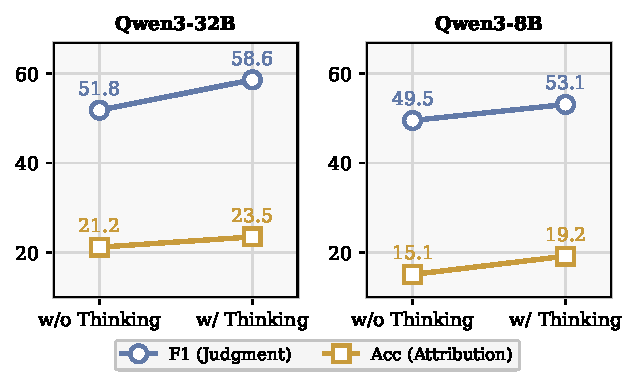
\includegraphics[width=1.0\linewidth]{Fig/thinking_comparison.pdf}
    \vspace{-1.6em}
    \caption{ The performance of judgment and attribution with and without thinking mode on Qwen3.
    }
    \label{fig:thinking_mode}
\end{figure}

\paragraph{Effect of Thinking Mode.}
We further study the effect of enabling thinking mode on automated hallucination judgment and attribution. Figure~\ref{fig:thinking_mode} shows consistent gains for both Qwen3 variants when thinking is enabled. For Qwen3-32B, judgment F1 improves from 51.8 to 58.6, while attribution accuracy increases from 21.2 to 23.5. The improvements are primarily attributable to enhanced self-verification under thinking mode, which better distinguishes plausible yet incorrect claims.

\begin{figure}[!ht]
  \centering
    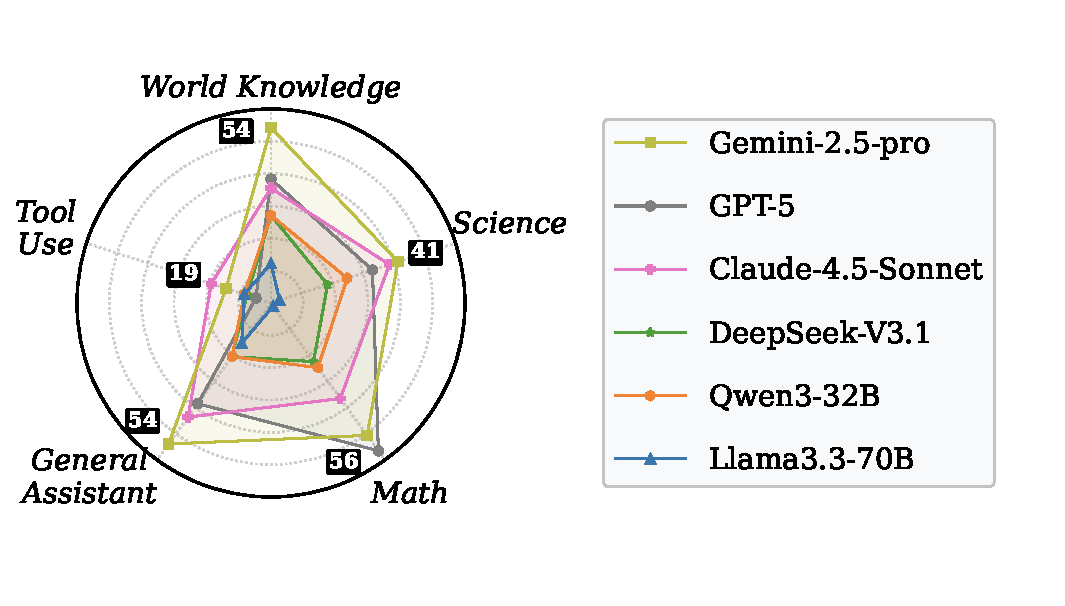
\includegraphics[width=1.0\linewidth]{Fig/agent_domain.pdf}
    \vspace{-1.6em}
    \caption{ Step localization accuracy of six evaluated LLMs across five domains.
    }
    \label{fig:agent_domain}
\end{figure}

\paragraph{Performance across Domains.}
We finally report step localization accuracy across five domains in Figure~\ref{fig:agent_domain}. The results show that attribution remains challenging across all models and varies substantially by domain. For knowledge-intensive queries, performance peaks on Math at 56\% accuracy but drops notably on Science to 41\% accuracy. Tool Use is consistently the hardest, suggesting current LLMs are challenging to precisely track environment states under sequential tool interactions.







